\documentclass{article}
\PassOptionsToPackage{table}{xcolor}
\usepackage{etoolbox}
\usepackage{qrcode}
\usepackage{geometry}
\geometry{a0paper,margin=1cm} % A0 portrait (841mm x 1189mm), per ICSSI 2026
\usepackage{graphicx}
\usepackage{enumitem}
\setlist{leftmargin=*,nosep,noitemsep}
\usepackage{anyfontsize}
% Roboto via fontspec (tectonic/XeTeX): loads the OTF files from the tectonic
% bundle by filename. Do NOT use [T1]{fontenc} here -- under XeTeX it forces a
% serif Latin Modern fallback instead of Roboto.
\usepackage{fontspec}
\setmainfont{Roboto}[
    Extension      = .otf,
    UprightFont    = *-Regular,
    BoldFont       = *-Bold,
    ItalicFont     = *-Italic,
    BoldItalicFont = *-BoldItalic,
]
\setsansfont{Roboto}[
    Extension      = .otf,
    UprightFont    = *-Regular,
    BoldFont       = *-Bold,
    ItalicFont     = *-Italic,
    BoldItalicFont = *-BoldItalic,
]
\renewcommand{\familydefault}{\sfdefault}
\usepackage{tikz}
\pagestyle{empty}
\usepackage{siunitx}
\usepackage{booktabs}
\sisetup{
        mode = match ,
        propagate-math-font = true ,
        reset-math-version = false ,
        reset-text-family = false ,
        reset-text-series = false ,
        text-family-to-math = true ,
        text-series-to-math = true ,
        range-phrase=\,--\,,
        group-separator={,},
        group-minimum-digits=3,
        group-digits=integer,
    }
\usepackage{caption}
\DeclareCaptionFormat{paper}{\fontsize{20pt}{25pt}\selectfont#1#2#3}
\captionsetup{format=paper}
\usepackage{xurl}
\usepackage{hyperref}
\hypersetup{hidelinks} % clickable but rendered as plain text (no boxes/recolor)
\urlstyle{same}
% Title, authors, affiliations, QR
    \newcommand{\dbtitle}{}        \renewcommand{\title}[1]{\renewcommand{\dbtitle}{#1}}
    \newcommand{\dbauthors}{}      \newcommand{\authors}[1]{\renewcommand{\dbauthors}{#1}}
    \newcommand{\dbaffiliations}{} \newcommand{\affiliations}[1]{\renewcommand{\dbaffiliations}{#1}}
    \newcommand{\dbQRcode}{} \newcommand{\QRcode}[1]{\renewcommand{\dbQRcode}{#1}}
    \newcommand{\dbQRcodeB}{} \newcommand{\QRcodeB}[1]{\renewcommand{\dbQRcodeB}{#1}}
%
    \usepackage[table]{xcolor}
    \definecolor{lightblue}{RGB}{189,215,238}
    \definecolor{medblue}{RGB}{141,180,226}
    \definecolor{darkblue}{RGB}{46,117,182}
    \definecolor{lightorange}{RGB}{248,203,173}
    \definecolor{medorange}{RGB}{244,176,132}
    \definecolor{darkorange}{RGB}{237,125,49}
% Colors (OSM forest-green scheme, shared with INCF poster)
    \definecolor{COLtitle}{HTML}{38761d}
    \definecolor{COL1}{HTML}{8cc793}
    \definecolor{COL2}{HTML}{6aa84f}
    \definecolor{COL3}{HTML}{799b5d}
    \definecolor{COL4}{HTML}{84cd34}
    \definecolor{COL5}{HTML}{6eaca2}
    \definecolor{COL6}{HTML}{69ba9f}
    \definecolor{COL7}{HTML}{83bcf0}
    \colorlet{COL1}{COLtitle}
    \colorlet{COL2}{COLtitle}
    \colorlet{COL3}{COLtitle}
    \colorlet{COL4}{COLtitle}
    \colorlet{COL5}{COLtitle}
    \colorlet{COL6}{COLtitle}
    \colorlet{COL7}{COLtitle}
% Poster environment (header / footer / body scaffold)
    \NewDocumentEnvironment{poster}{ +b }{\begin{tikzpicture}[remember picture,overlay,inner sep=0pt,outer sep=0pt]
        %
        % QR codes in the top corners (easy to photograph in a crowded hall)
        % Each QR (drawn [tight], i.e. no quiet-zone padding) has its descriptive
        % word on the line directly above and its link directly below, both in the
        % green title font.
        % NB: both the qrcode node and the \href link node carry extra phantom
        % box height, so neither .south nor a naive offset places the link
        % tightly. The link y-offset below is tuned empirically (against the
        % 5.5cm QR) so the link hugs the QR symmetrically with the label above.
        \node[anchor=north west] (QRL) at ([shift={(2cm,-2.7cm)}]current page.north west) {\qrcode[tight,height=5.5cm]{\dbQRcodeB}};
        \node[anchor=south,font=\fontsize{22pt}{24pt}\bfseries\color{COLtitle}\selectfont] at ([yshift=0.12cm]QRL.north) {Code \& Data};
        \node[anchor=north,font=\fontsize{16pt}{18pt}\bfseries\color{COLtitle}\selectfont] at ([yshift=-4.1cm]QRL.north) {\href{\dbQRcodeB}{10.5281/zenodo.20630081}};
        \node[anchor=north east] (QRR) at ([shift={(-2cm,-2.7cm)}]current page.north east) {\qrcode[tight,height=5.5cm]{\dbQRcode}};
        \node[anchor=south,font=\fontsize{22pt}{24pt}\bfseries\color{COLtitle}\selectfont] at ([yshift=0.12cm]QRR.north) {Dashboard};
        \node[anchor=north,font=\fontsize{16pt}{18pt}\bfseries\color{COLtitle}\selectfont] at ([yshift=-4.1cm]QRR.north) {\href{\dbQRcode}{opensciencemetrics.org}};
        % Institutional logos, inboard of the QR codes
        \node[anchor=north west] (LOGO) at ([shift={(1.5cm,0)}]QRL.north east) {
\includegraphics[width=8.5cm]{figures/NIH.png}};
        \node[anchor=north east] (LOGOR) at ([shift={(-1.5cm,0)}]QRR.north west) {
\includegraphics[width=8.5cm]{figures/DSST.png}};
        %
        \node[anchor=center,font=\fontsize{75pt}{85pt}\bfseries\color{COLtitle}\selectfont,text width=0.56\paperwidth,align=flush center] (TITLE) at (current page.north|-LOGO.center) {\dbtitle};
        \node[anchor=north,font=\fontsize{50pt}{60pt}\mdseries\color{black!50}\selectfont,text width=0.75\paperwidth,align=flush center] (AUTH) at ([yshift=-1cm]TITLE.south) {\dbauthors};
        \node[anchor=north,font=\fontsize{30pt}{40pt}\mdseries\color{black!50}\selectfont,text width=0.75\paperwidth,align=flush center] (AFFI) at ([yshift=-1cm]AUTH.south) {\dbaffiliations};
        % Rule
            \draw[COLtitle,line width=3pt] ([yshift=-1.5cm]current page.west|-AFFI.south) coordinate (Start) -- ([yshift=-1.5cm]current page.east|-AFFI.south);
        % Body
        #1
    \end{tikzpicture}}{}
% Poster box
\makeatletter
    \define@key{Pbox}{title}{\csdef{Ptitle}{#1}}
    \define@key{Pbox}{pos}{\csdef{Ppos}{#1}}
    \define@key{Pbox}{label}{\csdef{Plabel}{#1}}
    \define@key{Pbox}{color}{\csdef{Pcolor}{#1}}
    \define@key{Pbox}{width}{\csdef{Pwidth}{#1}}
\makeatother
\setkeys{Pbox}{}
\newlength{\Ppadding}\setlength{\Ppadding}{1cm}
\newlength{\Ptpadding}\setlength{\Ptpadding}{0.1cm}
\newlength{\Poffset}\setlength{\Poffset}{1cm}
\newcommand{\posterbox}[2][]{
    \csdef{Ptitle}{}
    \csdef{Ppos}{}
    \csdef{Plabel}{}
    \csdef{Pcolor}{}
    \csdef{Pwidth}{}
    \setkeys{Pbox}{#1}
    \node[anchor=north west,text width=\Pwidth,inner sep=\Ppadding,font=\fontsize{25pt}{30pt}\selectfont,align=flush left,draw=\Pcolor,line width=4pt,rounded corners=3pt] (\Plabel) at ([shift={(\Poffset,-2\Poffset)}]\Ppos) {\strut\\[-15pt]#2};
    \node[anchor=west,text=\Pcolor,fill=white,inner xsep=\Ptpadding,font=\fontsize{50pt}{50pt}\bfseries\selectfont] at ([xshift=\Ppadding-\Ptpadding]\Plabel.north west) {\MakeUppercase{\Ptitle}};
}

% Bibliography
\usepackage[backend=biber,style=science, maxcitenames=1, maxbibnames=1, isbn=false, sorting=none,doi=true,url=false]{biblatex}

\title{Who Funds Open Science? Tracking Data Sharing in Publications Across Major Funders}
\authors{Josh Lawrimore\textsuperscript{1}, Christoph Li\textsuperscript{2}, Dustin Moraczewski\textsuperscript{2}, Jean-Baptiste Poline\textsuperscript{3}, Adam Thomas\textsuperscript{2}}
\affiliations{\textsuperscript{1}Clinical Monitoring Research Program Directorate, Frederick National Laboratory for Cancer Research. \textsuperscript{2}Data Science \& Sharing Team, National Institute of Mental Health. \textsuperscript{3}Department of Neurology and Neurosurgery, McGill University.}
\QRcode{https://www.opensciencemetrics.org}                 % top-right: dashboard
\QRcodeB{https://doi.org/10.5281/zenodo.21042345}          % top-left: code & data (osm-icssi-2026 Zenodo concept DOI, always-latest)
\addbibresource{references.bib}
\begin{document}
\begin{poster}

    % ===================== LEFT COLUMN =====================
    \posterbox[
        title={Introduction},
        pos={Start},
        label={Intro},
        color={COL1},
        width={0.5\linewidth-2\Ppadding-\Poffset},
    ]{
        Open data sharing is central to the reproducibility and transparency of biomedical research, anchored by the FAIR principles for data stewardship~\cite{Wilkinson2016}. Funders, journals, and institutions increasingly \emph{mandate} sharing, yet measuring compliance at population scale remains difficult.
        \medskip

        Text mining XML versions of open-access articles systematically \emph{undercounts} data sharing because availability statements are often added late in production or appear in sections omitted from XML. In a landmark XML-based survey, open data rates reached only ${\sim}$15\% by 2020~\cite{Serghiou2021-pl}.
        \medskip

        We measured open data sharing across ${\sim}$784{,}000 recent biomedical articles using a \textbf{PDF-first} detection pipeline and benchmarked rates across major funders and journals.
    }

    \posterbox[
        title={Methods},
        pos={Intro.south-|Start},
        label={Methods},
        color={COL2},
        width={0.5\linewidth-2\Ppadding-\Poffset},
    ]{\begin{itemize}
        \item \num{784262} open access PubMed Central articles, January 2024 -- June 2025.
        \item Full text from \num{256660} PDFs (32.7\%) via \textbf{MinerU}~\cite{Wang2024mineru}; remaining \num{527602} (67.3\%) from PMC XML.
        \item Open data \& open code statements detected with \textbf{oddpub v7.2.3}~\cite{Riedel2020} via curated pattern matching.
        \item Funder, journal, and institution metadata from \textbf{OpenAlex}~\cite{Priem2022}; 816 funders normalized (e.g.\ NIH institutes aggregated to parent).
        \item \textbf{Major-funder filter (figure).} To compare peer agencies, the funders figure is restricted to funders with $\geq$\num{100000} total works indexed in OpenAlex \emph{and} above a Weibull-derived size threshold ($\geq$\num{2586} funded articles); the full ranking of all 816 funders is reported in the preprint.
        \item Observed rates are census-exact corpus proportions (no sampling interval). Journal-level \textbf{correction factors} from head-to-head PDF vs.\ XML comparison \emph{impute} the open-data statements PDF processing would have found on XML-only articles; the corrected estimate carries a 95\% Wilson-score \textbf{imputation interval}.
        \item Cross-sectional, descriptive design: reported differences are \emph{associations}, not causal policy effects.
        \item Recent mandates for data availability statements can lower the sensitivity of detection tools~\cite{Iarkaeva2024-wo}.
        \item All results explorable via an interactive dashboard at \texttt{opensciencemetrics.org}.
    \end{itemize}
    }

    \posterbox[
        title={Results: Funders},
        pos={Methods.south-|Start},
        label={ResultsFunders},
        color={COL5},
        width={0.5\linewidth-2\Ppadding-\Poffset},
    ]{
        \begin{center}
            
\includegraphics[width=\linewidth]{figures/funders_open_data_2024_2025.png}
        \end{center}
        \smallskip

        \textbf{Major biomedical funders}, ranked by open-data rate (see \emph{Methods} for the size filter). Solid bars: observed rate (PDF + XML); lighter bars: corrected estimate --- because mining XML alone misses data-availability statements present in the PDF, XML-only articles are adjusted upward using PDF-vs-XML correction factors; whiskers: 95\% imputation intervals on the corrected estimate (observed bars are census-exact, no interval); dashed line: 16.6\% funded-article baseline. Observed rates ranged from ${\sim}$10\% to ${\sim}$26\%: agencies with strong open-science cultures (ANR, the US and Swiss science foundations, Wellcome, DFG) reached up to ${\sim}$\textbf{1.6$\times$} the baseline, while the highest-volume funders (NSFC China, NIH) sat closer to it. Smaller and regional funders are excluded here, but several would rank at the very top --- e.g.\ the \emph{National Science Foundation of Sri Lanka} (27.7\%) and data-intensive research centers such as EMBL and SciLifeLab (45--53\%). The preprint ranks all 816 funders in full.
    }

    % ===================== RIGHT COLUMN =====================
    \posterbox[
        title={Takeaways},
        pos={Intro.east|-Start},
        label={Takeaways},
        color={COL4},
        width={0.5\linewidth-2\Ppadding-\Poffset},
    ]{\begin{itemize}
        \item Open-data rates varied \textbf{more than tenfold} across funders and journals.
        \item Open-data rate \textbf{8.7\%} across all articles, but \textbf{16.6\%} (${\sim}$2-fold) among articles that report funding.
        \item PDF-based detection found \textbf{${\sim}$52\% more} data-sharing statements than XML alone.
        \item Major funders reach observed rates above 20\% (corrected up to ${\sim}$28\%); top journals reach 70--86\% observed, with corrected estimates up to \textbf{92.9\%} (Nature Genetics).
        \item Data sharing rates vary \emph{consistently} by funder, helping funders identify which policies and practices most effectively incentivize sharing.
    \end{itemize}
    \smallskip
    \noindent
    \begin{minipage}[c]{0.80\linewidth}
        \begin{itemize}
            \item {\color{darkorange}\textbf{New result from ICSSI hackathon!}} Cross-checking our funder identification against \mbox{Dimensions'} fuller, publisher-sourced links, the ranking is largely robust (\mbox{Spearman}~0.88) --- though the \emph{European Commission} appears under-credited, rising to \#2 under more complete attribution.
        \end{itemize}
    \end{minipage}\hfill
    \begin{minipage}[c]{0.17\linewidth}\centering
        \qrcode[tight,height=2.6cm]{https://raw.githubusercontent.com/nimh-dsst/osm-icssi-2026/main/figures/funder_ranking_osm_vs_dim.png}\\[2pt]%
        {\fontsize{14pt}{15pt}\selectfont\color{COLtitle}\bfseries Scan to see\\ Dimensions figure\par}
    \end{minipage}
    }

    \posterbox[
        title={Results: Journals},
        pos={Takeaways.south-|Intro.east},
        label={ResultsJournals},
        color={COL5},
        width={0.5\linewidth-2\Ppadding-\Poffset},
    ]{
        \begin{center}
            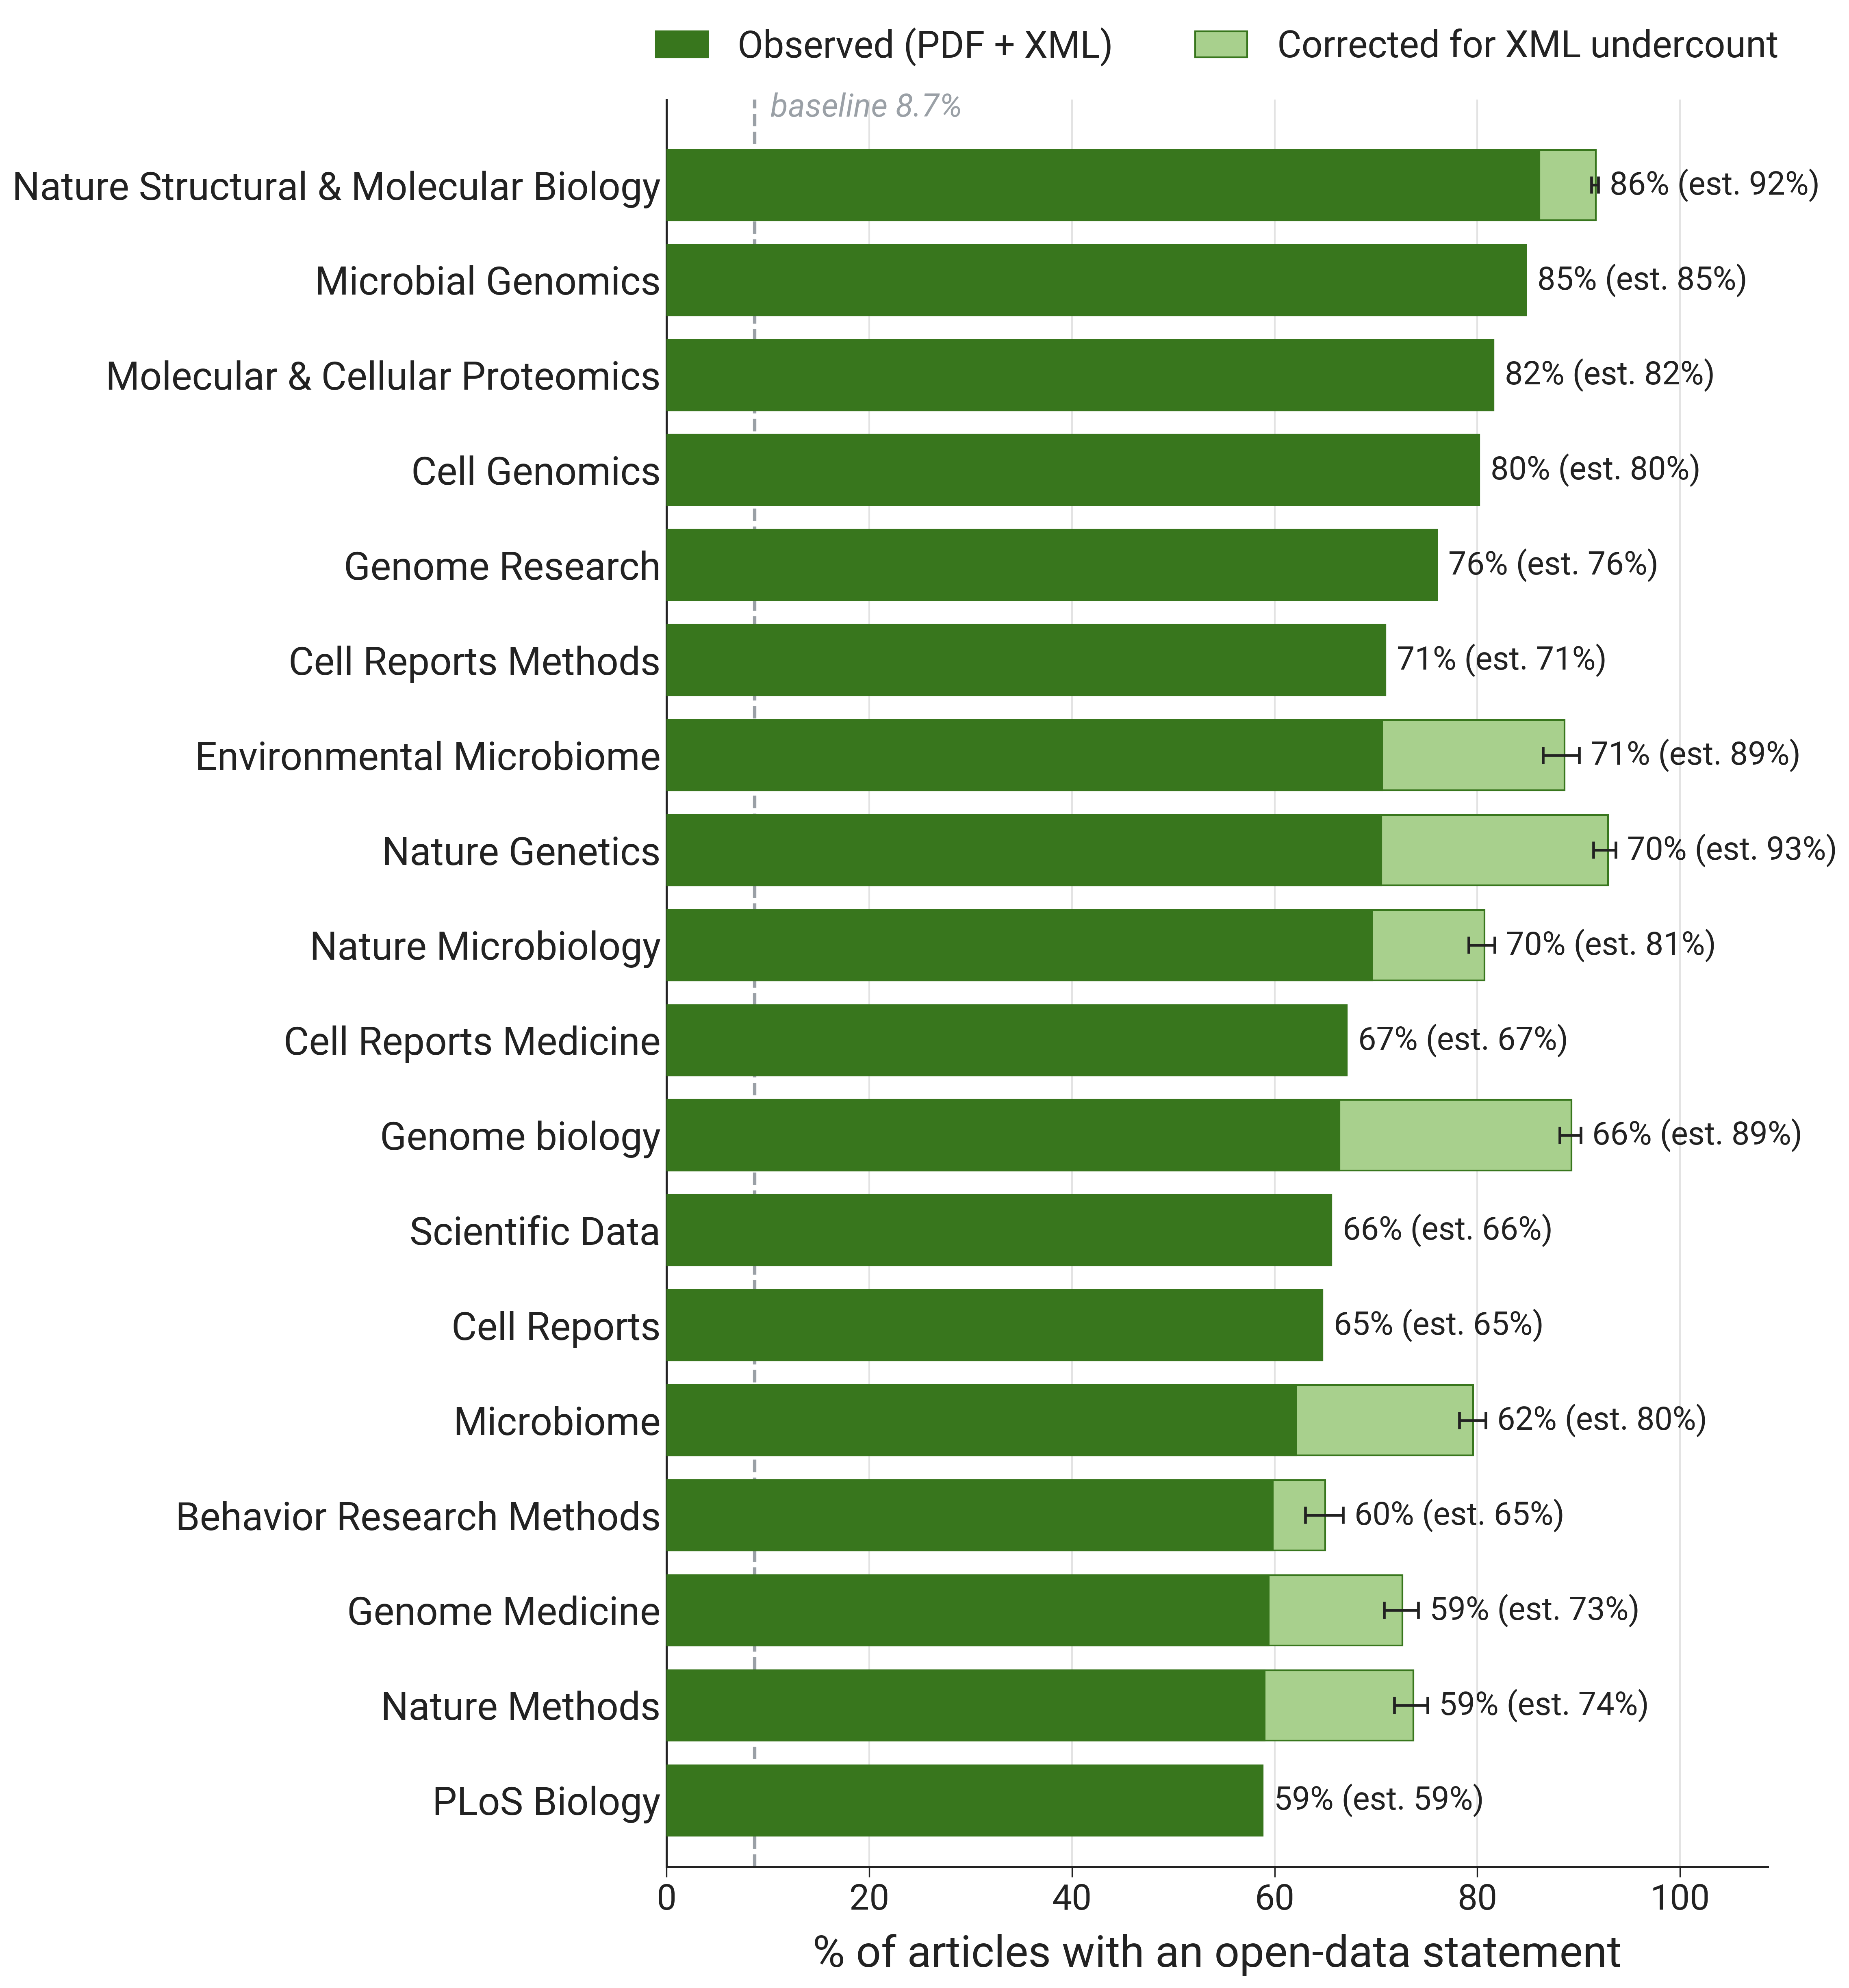
\includegraphics[width=\linewidth]{figures/journals_open_data_2024_2025.png}
        \end{center}
        \smallskip

        \textbf{The 18 highest-rate journals} ($\geq$150 articles). Bars, whiskers, and shading as in the funders figure; lighter bars use journal-level correction factors from head-to-head PDF vs.\ XML comparison; dashed line: 8.7\% overall baseline. Across all 1{,}389 journals, rates spanned below 5\% to above 90\%. The leaders shown here are dominated by genomics and structural-biology titles, with psychology methods journals (e.g.\ \emph{Behavior Research Methods}) also prominent --- reflecting post-replication-crisis norms.
    }

    \posterbox[
        title={Discussion},
        pos={ResultsJournals.south-|Intro.east},
        label={Discussion},
        color={COL6},
        width={0.5\linewidth-2\Ppadding-\Poffset},
    ]{\begin{itemize}
        \item Variation clusters by \textbf{disciplinary norms} (genomics and psychology journals lead) and by funder/journal policy \textbf{stringency and enforcement} --- not the mere existence of a mandate.
        \item Detecting a \emph{statement} is not the same as verifying \emph{accessible} data; reported rates are upper bounds. External validation suggests current rates are conservative~\cite{Deeb2025-iw}.
        \item Because funders and journals are not randomly assigned to articles, differences reflect a confounded mix of policy, discipline, infrastructure, and self-selection.
        \item \textbf{Future work:} expand PDF coverage and extend the window to enable longitudinal analysis of policy changes (e.g.\ the 2023 NIH Data Management \& Sharing Policy).
    \end{itemize}
    }

    % ===================== BOTTOM BOXES =====================
    % Each continues its own column at the shared 0.5-width grid: References
    % below the funders figure (left), Acknowledgments & Funding below
    % Discussion (right), so the latter fills the gap under Discussion.
    \posterbox[
        title={References},
        pos={ResultsFunders.south-|Start},
        label={References},
        color={COL3},
        width={0.5\linewidth-2\Ppadding-\Poffset},
    ]{\AtNextBibliography{\fontsize{14pt}{17pt}\selectfont}\printbibliography[heading=none]}

    \posterbox[
        title={Acknowledgments \& Funding},
        pos={Discussion.south-|Intro.east},
        label={AckFunding},
        color={COL7},
        width={0.5\linewidth-2\Ppadding-\Poffset},
    ]{\fontsize{17pt}{21pt}\selectfont
        We thank John Lee, Travis Riddle, David Siedband, Jason Priem, Heather Piwowar, Kendra Oudyk, Francisco Pereira, Juan Antonio Lossio-Ventura, David Kennedy, and the Tanenbaum Open Science Institute (TOSI) for contributions, comments, and support on earlier versions of this project. This work used the NIH HPC Biowulf cluster (\texttt{hpc.nih.gov}).
        \smallskip

        \textbf{Generative AI.} The authors used generative AI tools (Anthropic's Claude, OpenAI models, the Cursor editor) as drafting, editing, and coding assistants. All numerical results were verified against the underlying analysis outputs. Generative AI was not used to fabricate, alter, or substitute for the underlying data.
        \smallskip

        \textbf{Funding.} This research was supported in part by the Intramural Research Program of the National Institutes of Health (NIH). The contributions of the NIH author(s) were made as part of their official duties as NIH federal employees, are in compliance with agency policy requirements, and are considered Works of the United States Government. However, the findings and conclusions presented in this paper are those of the author(s) and do not necessarily reflect the views of the NIH or the U.S.\ Department of Health and Human Services (HHS). NIH support was provided under NIMH project ZICMH002960. This project was also funded in whole or in part with federal funds from the National Cancer Institute, NIH, under Contract No.\ 75N91019D00024; mention of trade names, commercial products, or organizations does not imply endorsement by the U.S.\ Government.\par
    }

\end{poster}
\end{document}
